\documentclass{beamer}
\beamertemplatenavigationsymbolsempty
\usecolortheme{beaver}
\setbeamertemplate{blocks}[rounded=true, shadow=true]
\setbeamertemplate{footline}[page number]
%
% packages
\usepackage{amsmath,amssymb}
\usepackage{graphicx}
\usepackage{hyperref}

% directory of figures
%\graphicspath{ {figs} }

% latin bold lower
\newcommand{\ba}{\mathbf{a}}
\newcommand{\bc}{\mathbf{c}}
\newcommand{\be}{\mathbf{e}}
\newcommand{\bh}{\mathbf{h}}
\newcommand{\bp}{\mathbf{p}}
\newcommand{\bt}{\mathbf{t}}
\newcommand{\bs}{\mathbf{s}}
\newcommand{\bu}{\mathbf{u}}
\newcommand{\bv}{\mathbf{v}}
\newcommand{\bw}{\mathbf{w}}
\newcommand{\bx}{\mathbf{x}}
\newcommand{\by}{\mathbf{y}}
\newcommand{\bz}{\mathbf{z}}
\newcommand{\bm}{\mathbf{m}}

% latin bold upper
\newcommand{\bA}{\mathbf{A}}
\newcommand{\bB}{\mathbf{B}}
\newcommand{\bC}{\mathbf{C}}
\newcommand{\bI}{\mathbf{I}}
\newcommand{\bJ}{\mathbf{J}}
\newcommand{\bL}{\mathbf{L}}
\newcommand{\bM}{\mathbf{M}}
\newcommand{\bP}{\mathbf{P}}
\newcommand{\bQ}{\mathbf{Q}}
\newcommand{\bR}{\mathbf{R}}
\newcommand{\bT}{\mathbf{T}}
\newcommand{\bU}{\mathbf{U}}
\newcommand{\bV}{\mathbf{V}}
\newcommand{\bW}{\mathbf{W}}
\newcommand{\bX}{\mathbf{X}}
\newcommand{\bY}{\mathbf{Y}}
\newcommand{\bZ}{\mathbf{Z}}

% latin cal upper
\newcommand{\cF}{\mathcal{F}}
\newcommand{\cG}{\mathcal{G}}
\newcommand{\cI}{\mathcal{I}}
\newcommand{\cL}{\mathcal{L}}
\newcommand{\cM}{\mathcal{M}}
\newcommand{\cN}{\mathcal{N}}
\newcommand{\cS}{\mathcal{S}}
\newcommand{\cT}{\mathcal{T}}
\newcommand{\cW}{\mathcal{W}}
\newcommand{\cX}{\mathcal{X}}
\newcommand{\cZ}{\mathcal{Z}}

% latin bb upper
\newcommand{\bbE}{\mathbb{E}}
\newcommand{\bbI}{\mathbb{I}}
\newcommand{\bbP}{\mathbb{P}}
\newcommand{\bbR}{\mathbb{R}}
\newcommand{\bbX}{\mathbb{X}}
\newcommand{\bbY}{\mathbb{Y}}
\newcommand{\bbW}{\mathbb{W}}

% greek bold lower
\newcommand{\bepsilon}{\boldsymbol{\epsilon}}
\newcommand{\btheta}{\boldsymbol{\theta}}
\newcommand{\blambda}{\boldsymbol{\lambda}}
\newcommand{\bpi}{\boldsymbol{\pi}}
\newcommand{\bmu}{\boldsymbol{\mu}}
\newcommand{\bsigma}{\boldsymbol{\sigma}}
\newcommand{\bphi}{\boldsymbol{\phi}}

% greek bold upper
\newcommand{\bSigma}{\boldsymbol{\Sigma}}

\DeclareMathOperator*{\argmin}{arg\,min}
\DeclareMathOperator*{\argmax}{arg\,max}

% transpose
\newcommand{\T}{^{\text{\tiny\sffamily\upshape\mdseries T}}}

%
\usepackage[utf8]{inputenc}
\usepackage[english]{babel}
\usepackage{amssymb,amsfonts,amsmath,mathtext}
\usepackage{subfig}
\usepackage[all]{xy}
\usepackage{array}
\usepackage{multicol}
\usepackage{hyperref}
\usepackage{tabularx}   
\usepackage{hhline}

\setbeamertemplate{itemize item}{}
\setbeamertemplate{itemize subitem}{}
\setbeamertemplate{itemize subsubitem}{}

%----------------------------------------------------------------------------------
\title[Loss Landscape Convergence]{Neural Networks Loss Landscape Convergence in Hessian Low-Dimensional Space}
\author[Tem Nikitin \textit{et al.}]{Tem Nikitin, Nikita Kiselev, Vladislav Meshkov, Andrey Grabovoy}
\institute{Moscow Institute of Physics and Technology}
\date{2025}
%----------------------------------------------------------------------------------
\begin{document}

\begin{frame}
    \thispagestyle{empty}
    \maketitle
\end{frame}

\begin{frame}{Neural Networks Loss Landscape Convergence in Hessian Low-Dimensional Space}
    \textbf{Goals and Tasks}
    \begin{enumerate}
        \item Study how neural network loss landscape changes with dataset size
        \item Define and measure metrics $\Delta_k$
        \item Derive theoretical bound for $\Delta_k$ via top-$d$ eigenvalues
        \item Propose an algorithm to determine the $\Delta$-sufficient dataset size
    \end{enumerate}
\end{frame}

\begin{frame}{Loss landscape stabilizes after sufficient sample size.}
    \begin{columns}[c]
        \hspace{-1.5cm}
        \column{0.6\textwidth}
        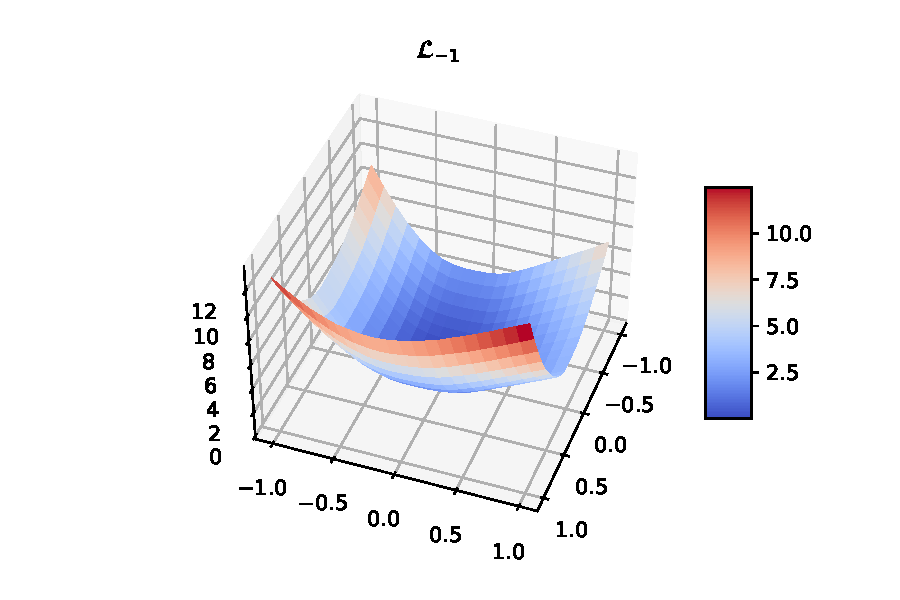
\includegraphics[width=1.34\textwidth]{img/loss_eigen_-1_individ.pdf}
        \column{0.5\textwidth}
        \begin{itemize}
            \item Hessian projection onto top-$d$ eigenvectors
            \item Monte Carlo estimate of $\Delta_k^{emp} = \mathbb{E} \Bigl( \cL_{k+1} - \cL_{k} \Bigr)^2.$
            \item Analytical bound: $\Delta_k^{th} \ge \Delta_k^{emp}$
            \item Detect dataset threshold $k^*$
        \end{itemize}
    \end{columns}
\end{frame}

\begin{frame}{Problem Statement}
    \begin{block}{Hypothesis}
        Beyond some $k^*$, adding new samples changes the local loss landscape by less than a tolerance $\Delta_{tol}$, i.e.
        $\forall\, k \ge k^* : \; \Delta_k < \Delta_{tol}$.
    \end{block}
    \begin{block}{Model}
        \begin{itemize}
            \item MLP with ReLU activations for $K$-class classification
            \item Empirical loss: $\cL_k(\bw) = \frac1k \sum_{i=1}^k \ell_i(\bw)$
            \item Hessian: $\bH_k(\bw) = \nabla^2_{\bw} \cL_k(\bw)$
        \end{itemize}
    \end{block}

    \begin{block}{Criteria}
        \begin{itemize}
            \item Convergence rate: $\Delta_k = O(1/k^2)$
            \item Theoretical bound via top-$d$ eigenvalues upper-bounds empirical $\Delta_k$
            \item Plateau in eigenvalue differences $\lambda_i^{k+1}-\lambda_i^k$ indicates threshold
        \end{itemize}
    \end{block}
\end{frame}


\begin{frame}{Theoretical Analysis}
    \begin{columns}[c]
        \column{0.4\textwidth}
        \begin{itemize}
            \item Project parameters: $\bw = \bw^* + \bP \btheta$, $\bP = [\be_1, \dots, \be_d]$
            \item Taylor approx: $\cL_k (\bw^* + \bP \btheta) \approx \cL_k (\bw^*) + \tfrac12 \btheta^{\T} \bLambda_k \btheta$
                  \bigskip
                  \bigskip
        \end{itemize}
        \column{0.8\textwidth}
        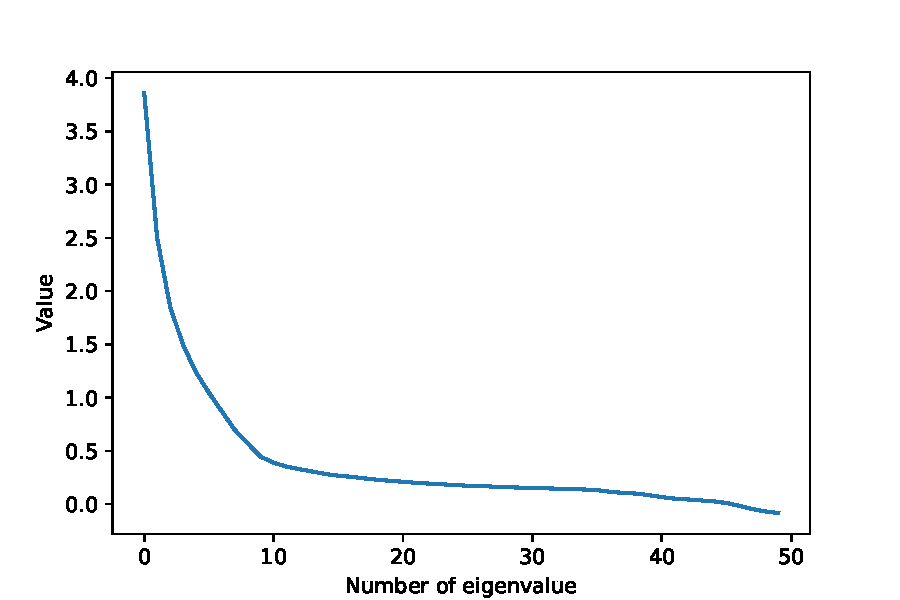
\includegraphics[width=1.0\textwidth]{img/eigenvalues.pdf}
        \vspace{0.5cm}\hspace{3.1cm}\raggedright{Eigenvalue decay}
    \end{columns}
    Bound:
    $ \Delta_k \approx
        \frac{\sigma^4}{4}\, \Biggl( 2 \sum_{i=1}^d (\lambda_{k+1}^i - \lambda_k^i)^2
        + \Bigl( \sum_{i=1}^d (\lambda_{k+1}^i - \lambda_k^i) \Bigr)^2 \Biggr).$
\end{frame}

\begin{frame}{Computational Experiment}
    \begin{itemize}
        \item Datasets: MNIST, Fashion-MNIST (60k train, 10k test)
        \item MLP: 2 hidden layers, $\sim 10^5$ parameters
        \item Subspace dimension $d=10$, Monte Carlo samples $K=64$, $\sigma=1$
        \item Compare empirical $\Delta_k$ vs theoretical bound across $k$
    \end{itemize}

    \begin{figure}
        \centering
        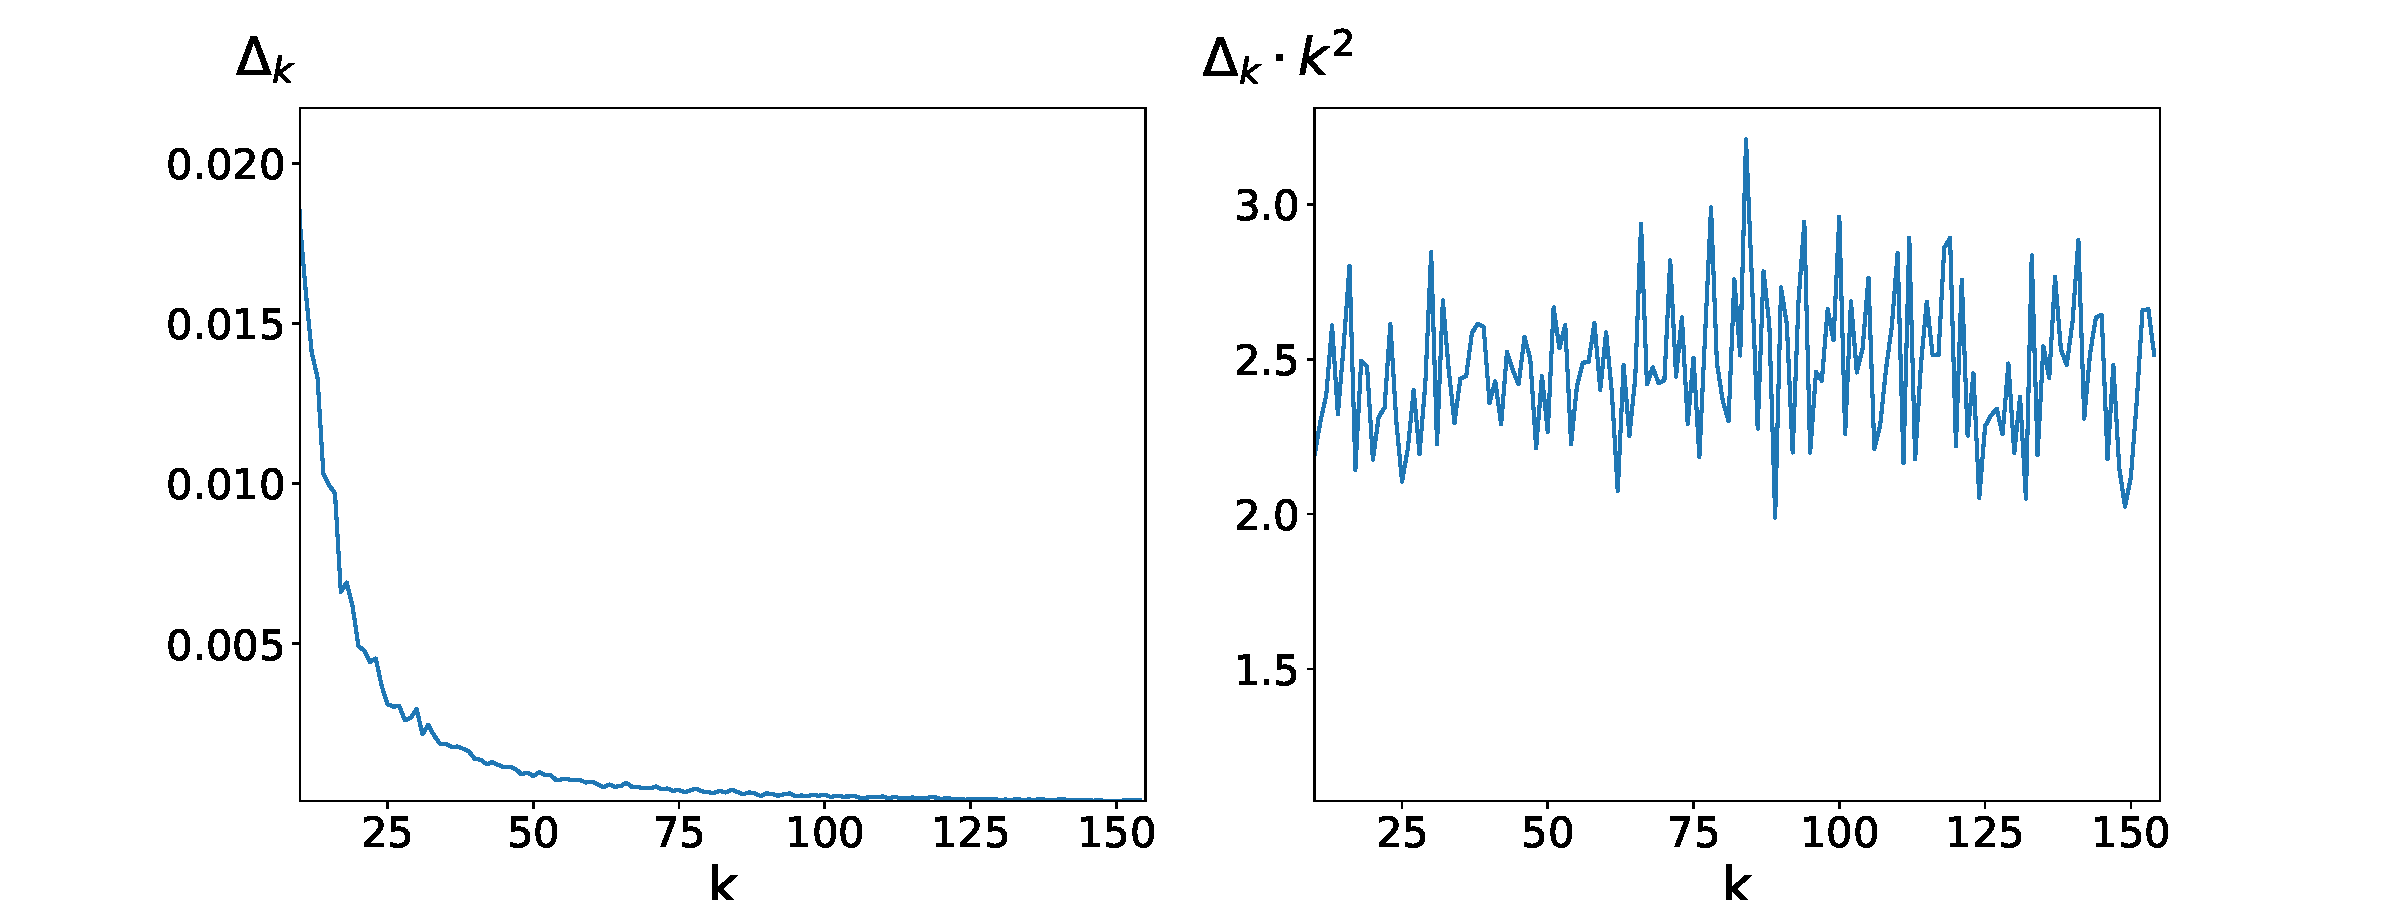
\includegraphics[width=1.05\textwidth,trim=0 17 0 1.5cm,clip]{img/delta_eigen_1_10_1024.pdf}
        \caption*{Monte Carlo $\Delta_k$ vs $k$ and $\Delta_k\cdot k^2$}
    \end{figure}
\end{frame}

\begin{frame}{Combining results}
    \begin{itemize}
        \item Empirical $\Delta_k$ consistently below theoretical estimate
        \item Gap due to neglected eigen-modes beyond top-$d$
        \item Monte Carlo variance decreases with sample size $K$
    \end{itemize}

    \begin{figure}
        \centering
        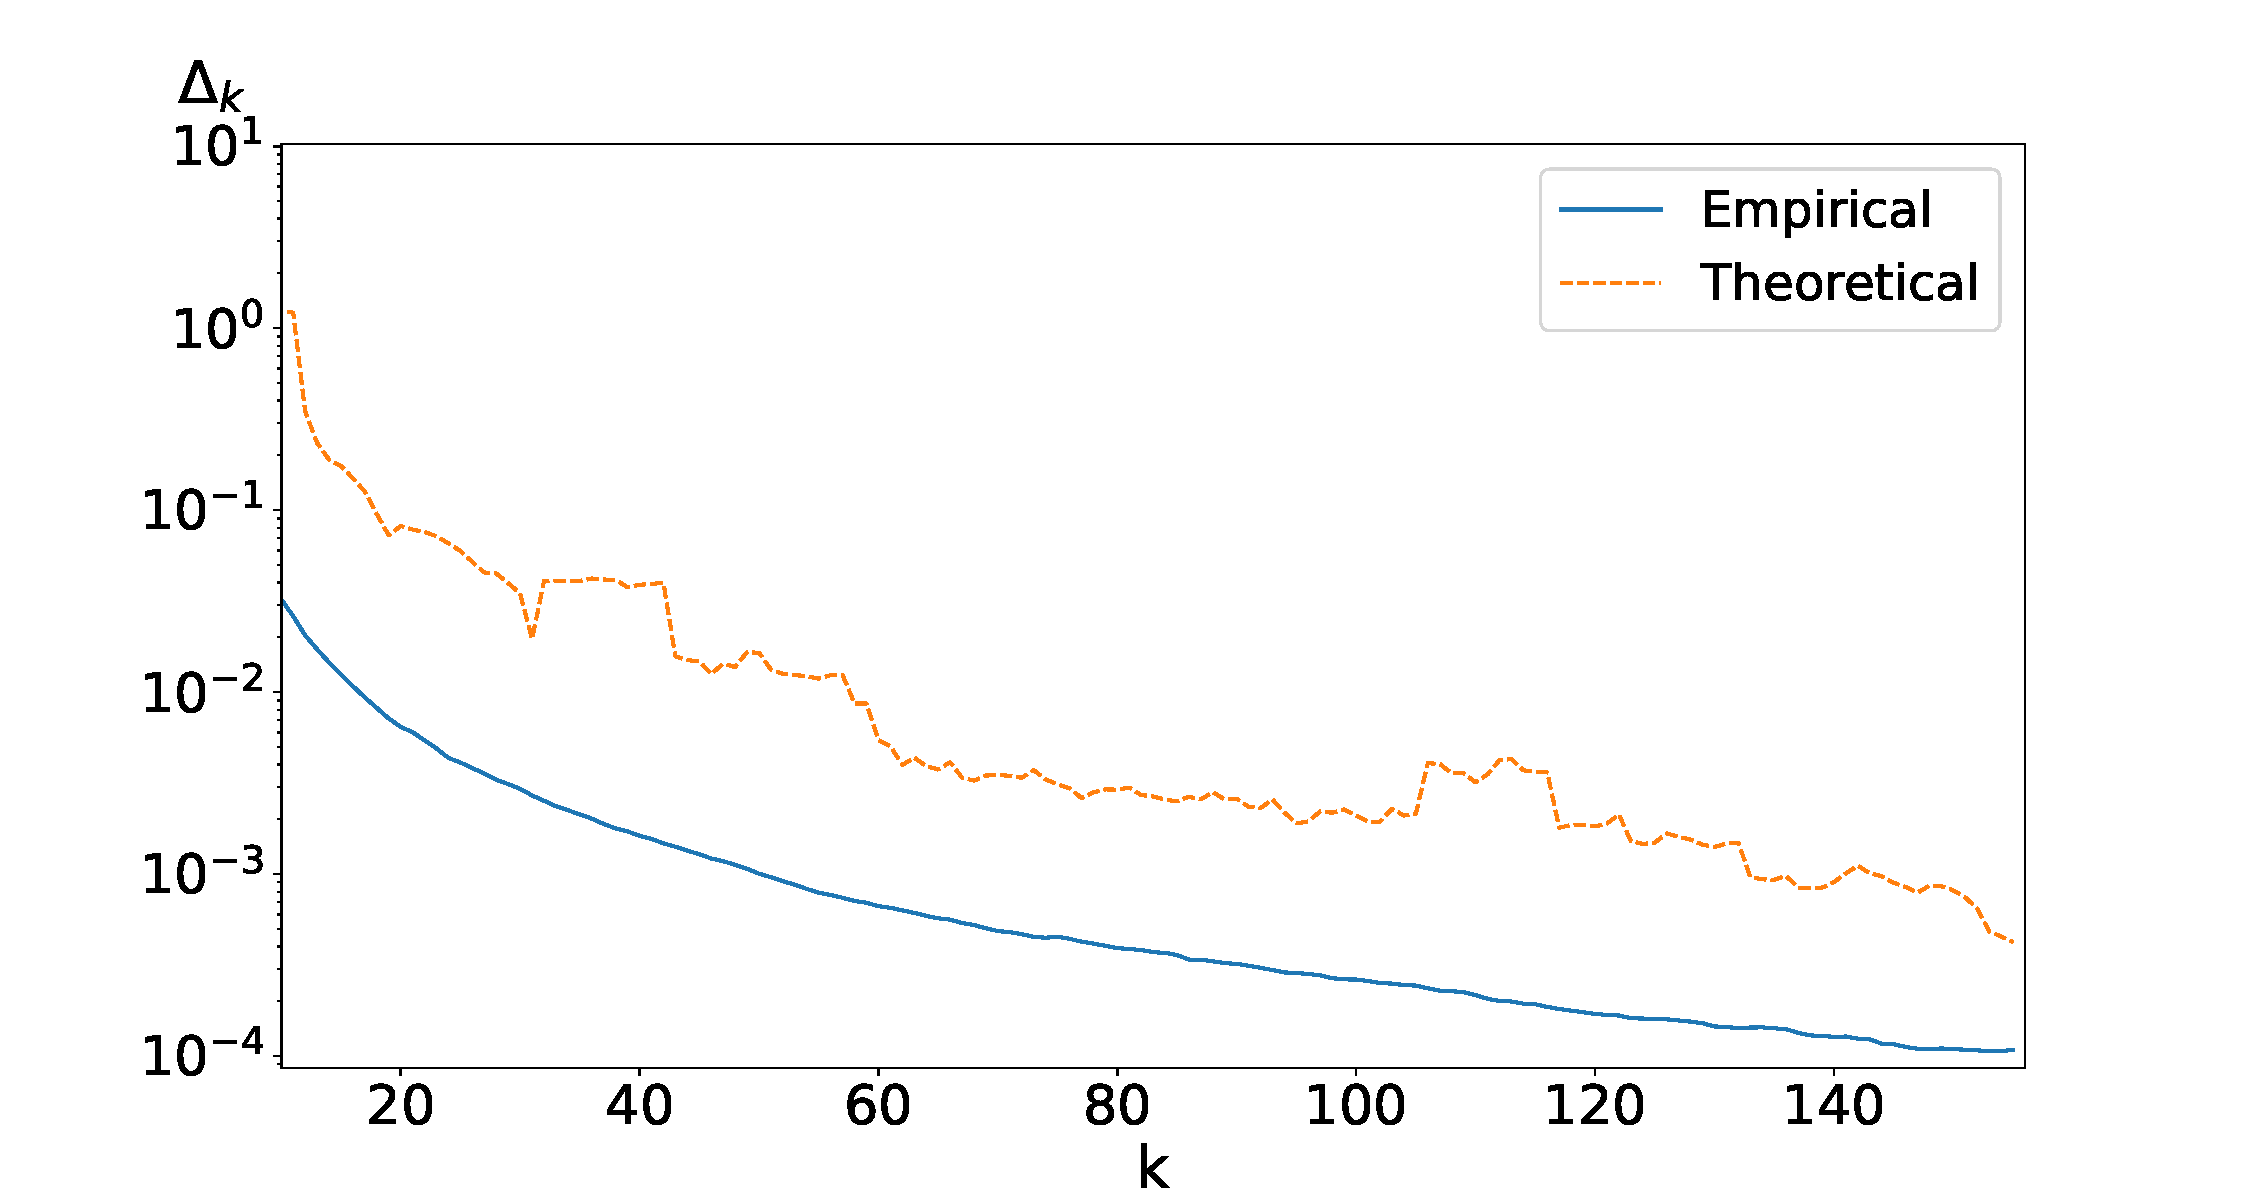
\includegraphics[width=0.9\textwidth]{img/delta_border_1_10_1024.pdf}
        \caption*{Theoretical (dashed) vs empirical (solid) $\Delta_k$}
    \end{figure}
\end{frame}

\begin{frame}{Theoretical vs. Empirical $\Delta_k$}
    \begin{figure}
        \centering
        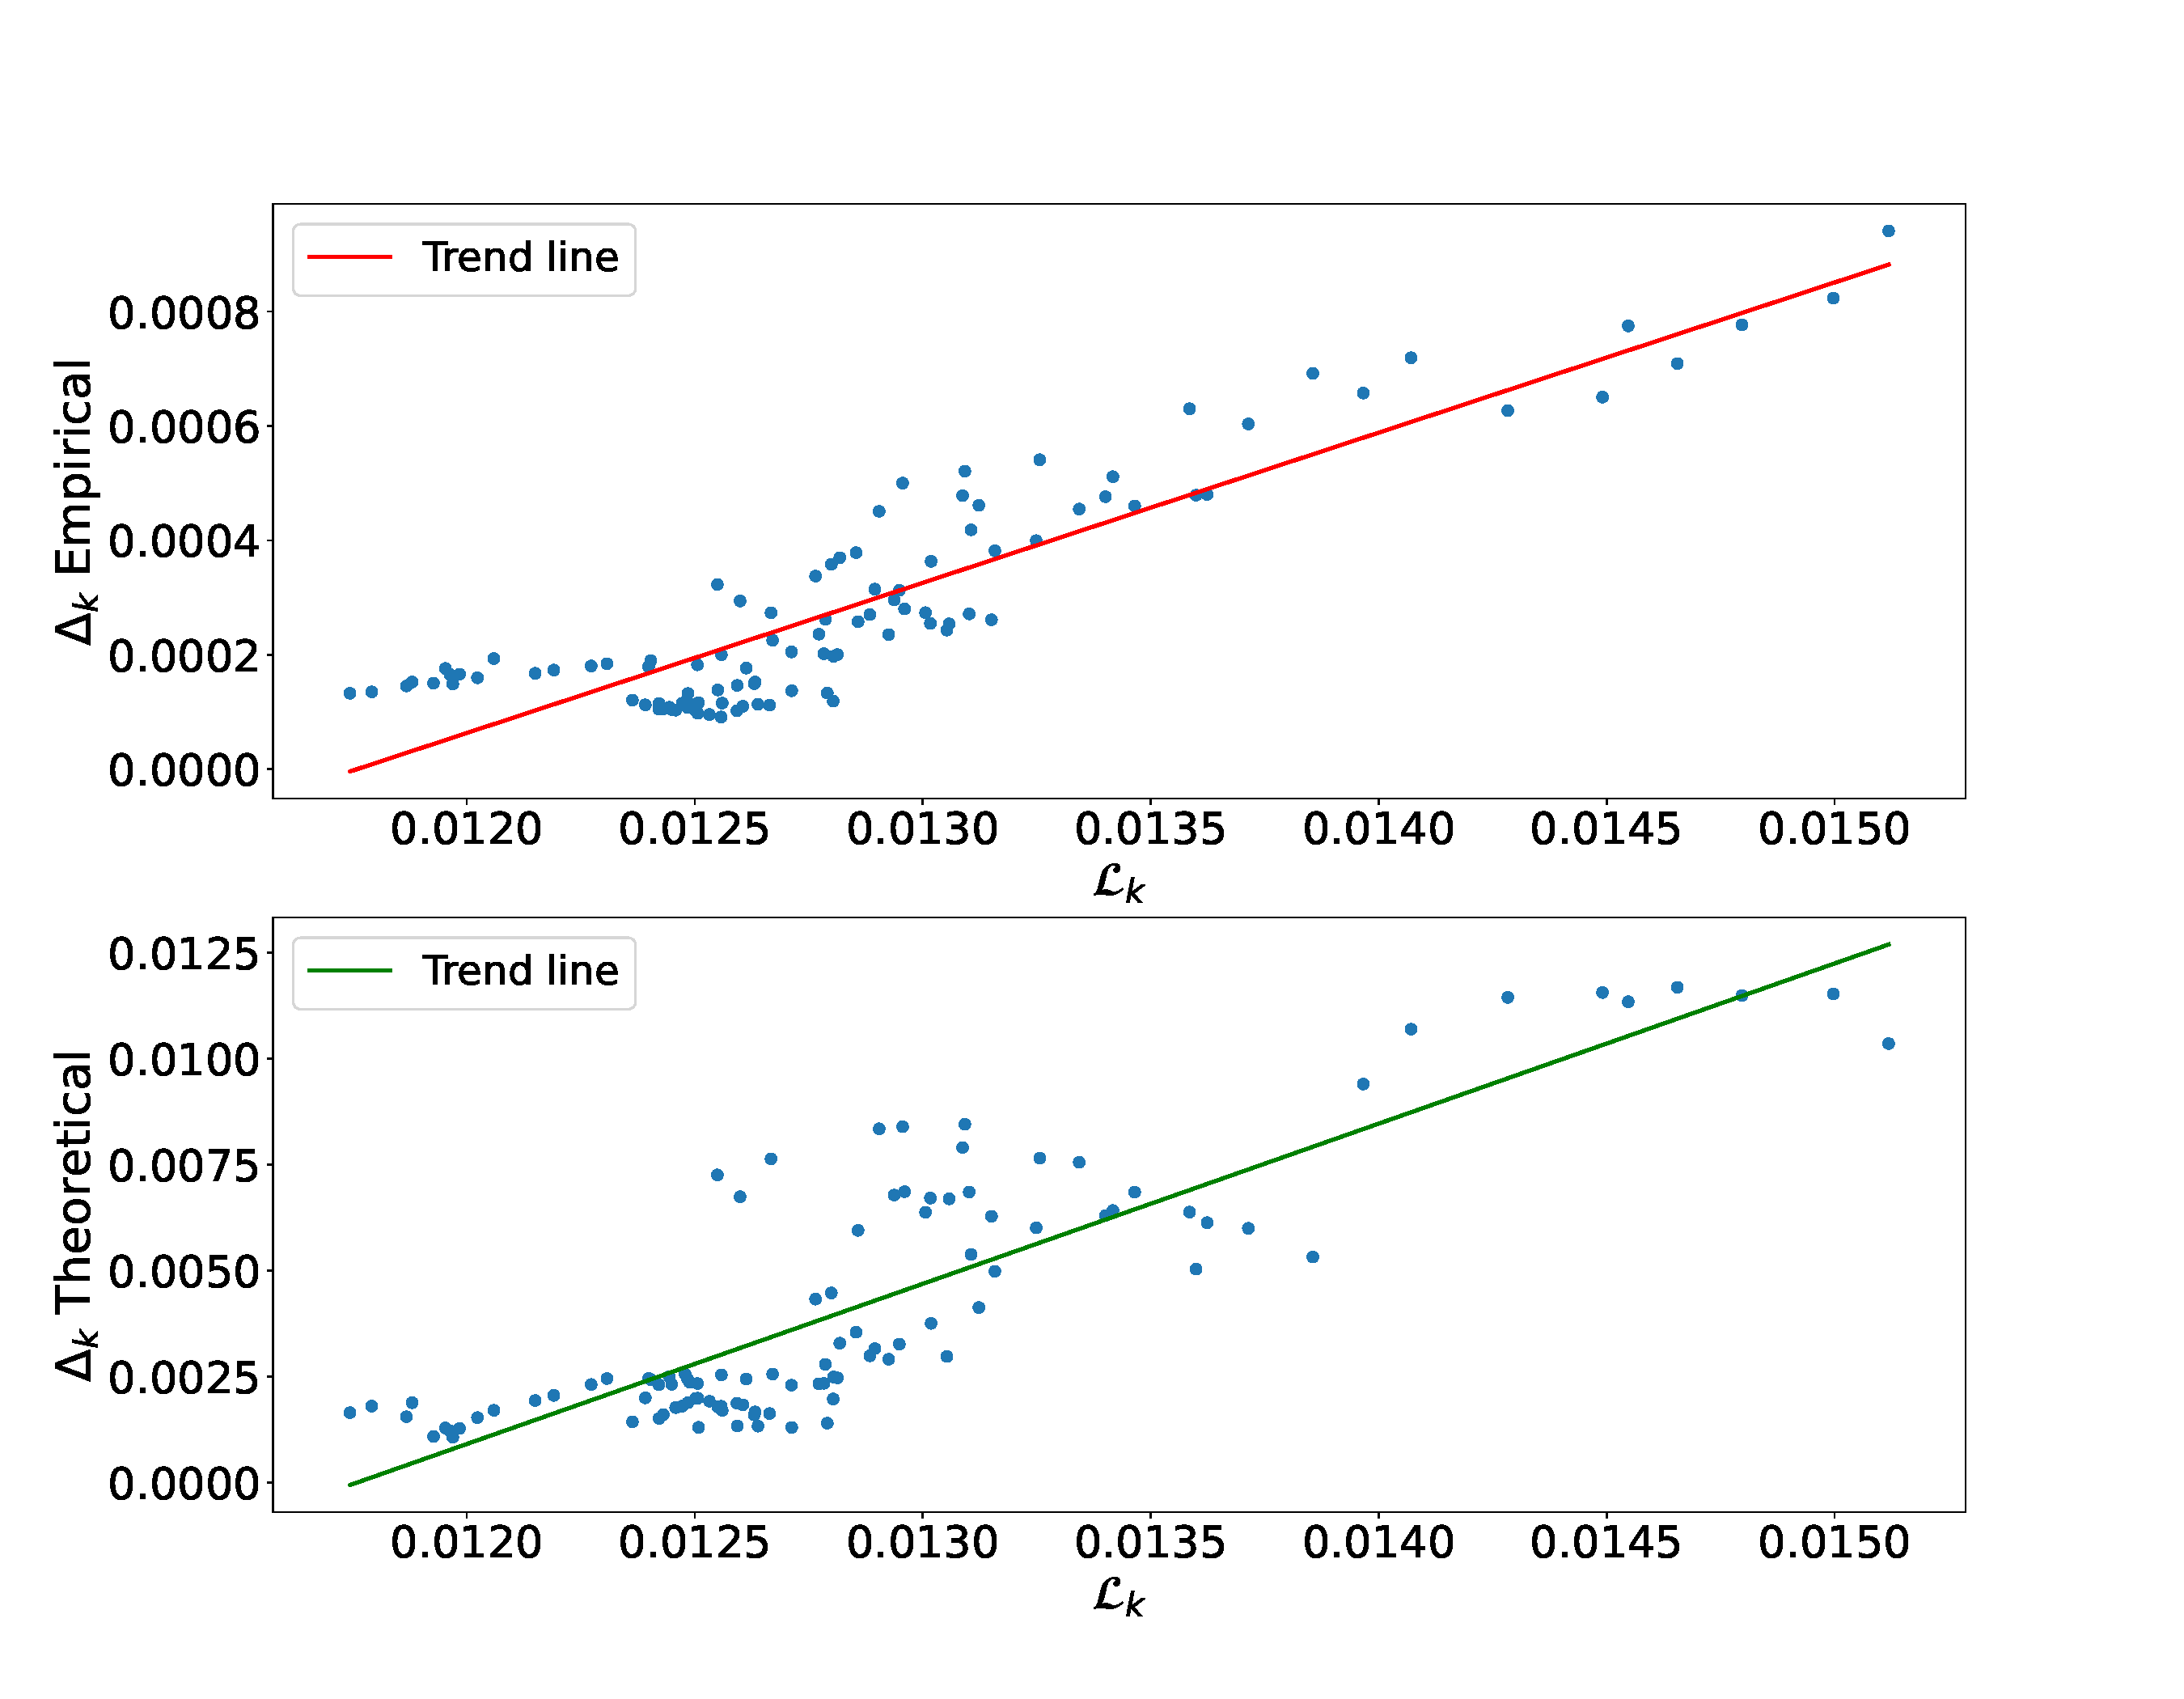
\includegraphics[width=1\textwidth]{img/delta_loss_1_10_1024.pdf}
    \end{figure}
\end{frame}


\begin{frame}{Practical Measurements}
    \begin{table}
        \centering
        \small
        \begin{tabularx}{\textwidth}{|l|>{\raggedright\arraybackslash}X|c|c|c|c|}
            \hline
            \textbf{Dataset}
                          & \textbf{Model}    & \(\Delta\) & \(k\) & \(L_k\) & \textbf{Time (s)} \\
            \hhline{|=|=|=|=|=|=|}
            MNIST         & Single-layer MLP  & 0.025      & 100   & 0.013   & 2000              \\
                          & Multi-layer MLP   & 0.025      & 40    & 0.010   & 3500              \\
                          & Convolutional CNN & 0.025      & 60    & 0.024   & 1800              \\
            \hline
            Fashion-MNIST & Single-layer MLP  & 0.030      & 120   & 0.020   & 2100              \\
                          & Multi-layer MLP   & 0.030      & 90    & 0.017   & 4400              \\
                          & Convolutional CNN & 0.030      & 70    & 0.015   & 2400              \\
            \hline
        \end{tabularx}
    \end{table}
\end{frame}

\begin{frame}{Algorithm: \(\Delta\)-sufficient Dataset Size}
    \begin{block}{Algorithm 1: Determine \(\Delta\)-sufficient dataset size}
        \begin{enumerate}
            \item Initialize dataset \(D \gets \emptyset\) and batch counter \(k \gets 0\).
            \item \textbf{Repeat:}
                  \begin{itemize}
                      \item \(k \gets k + 1\).
                      \item Sample a new batch of data and append to \(D\).
                      \item Train or update model on \(D\).
                      \item Compute top-\(d\) Hessian eigenvalues \(\{\lambda_k^{(i)}\}_{i=1}^d\) and \(\{\lambda_{k+1}^{(i)}\}\).
                      \item Estimate
                            \[
                                \Delta_k \approx \frac{\sigma^4}{4}\Bigl(2\sum_{i=1}^d(\lambda_{k+1}^{(i)}-\lambda_k^{(i)})^2
                                + \bigl(\sum_{i=1}^d(\lambda_{k+1}^{(i)}-\lambda_k^{(i)})\bigr)^2\Bigr).
                            \]
                  \end{itemize}
            \item \textbf{Until} \(\Delta_k < \Delta_{\text{tol}}\).
            \item \textbf{Return} \(|D|\), the \(\Delta\)-sufficient sample size.
        \end{enumerate}
    \end{block}
\end{frame}

\begin{frame}{Results and Conclusions}
    \begin{enumerate}
        \item Identified dataset thresholds \(k^*\) for MNIST and Fashion-MNIST.
        \item Loss landscape stabilizes: additional data negligible beyond \(k^*\).
        \item Hessian-based bound provides a reliable upper-bound for \(\Delta_k\).
        \item Proposed a practical algorithm for \(\Delta\)-sufficient dataset sizing.
        \item Offers guidelines for dataset collection and early stopping.
    \end{enumerate}
\end{frame}

\begin{frame}{Literature}
    \begin{enumerate}
        \item Wu \textit{et al.} (2017): loss landscapes vs dataset size
        \item Sagun \textit{et al.} (2018): Hessian low effective rank
        \item Li \textit{et al.} (2018): visualizing loss surfaces
        \item Ghorbani \textit{et al.} (2019): eigenvalue density analysis
        \item Bousquet \& Elisseeff (2002): stability and generalization bounds
    \end{enumerate}
\end{frame}

\end{document}
